\section{Task Description: Alignment to Reference Graphs} \label{TRIEsec:task}

We now describe the task of aligning a query to a reference graph. To this end,
we (i)~introduce the task of optimal alignment on a \emph{reference graph},
(ii)~formalize this task in terms of an \emph{edit graph}, and (iii)~introduce an
alternative formulation in terms of an \emph{alignment graph}, which is the
basis for shortest path formulations of the optimal alignment.
%
\cref{TRIEfig:graph-constructions} summarizes these different graph types.

\para{Reference Graph}
We encode the collection of references to which we want to align in a reference
graph, which captures genomic variation that a linear reference cannot
express~\cite{paten_genome_2017,garrison_variation_2018}.
%
We formalize a reference graph as a tuple $\RG=(\RGV,\RGE)$ of nodes $\RGV$ and
directed, labeled edges $\RGE \subseteq \RGV \times \RGV \times \Sigma$, where
the alphabet $\Sigma=\{\texttt{A},\texttt{C},\texttt{G},\texttt{T}\}$ represents
the four different nucleotides.
%
Note that in contrast to sequence graphs~\cite{rautiainen_aligning_2017}, we
label edges instead of nodes.

\para{Path, Spelling}
Any path $\pi=(e_1,\dots,e_k) \text { in } \RG$ induces a \emph{spelling}
$\sigma(\pi) \in \Sigma^*$ defined by $\sigma(e_1)\cdots\sigma(e_k)$, where
$\sigma(e_i)$ is the label of edge $e_i$ and $\Sigma^* := \bigcup_{k \in
\mathbb{N}} \Sigma^k$. We note that our approach naturally handles cyclic walks
and does not require cycle unrolling, a feature shared with
\bitparallel~\cite{rautiainen_bitparallel_2019} and
\brownie~\cite{heydari_browniealigner_2018} but missing from
\vg~\cite{garrison_variation_2018}, \pasgal~\cite{jain_accelerating_2019} and
\valigntool~\cite{kavya_sequence_2019}.

\para{Alignment on Reference Graph}
An \emph{alignment} of \emph{query} $q \in \Sigma^*$ to a reference graph
$\RG=(\RGV,\RGE)$ consists of (i)~a path $\pi \text{ in } \RG$ and (ii)~a
sequence of edit operations (matches, substitutions, insertions, deletions)
transforming $\sigma(\pi)$ to~$q$.

\para{Optimal Alignment, Edit Distance}
Each edit operation is associated with a real-valued cost ($\cmatch$, $\csubst$,
$\cins$, and $\cdel$, respectively).
An optimal alignment minimizes the total cost of the edit operations converting
$\sigma(\pi)$ to $q$. For optimal alignments, this total cost is equal to the
edit distance between $\sigma(\pi)$ and $q$, \ie, the cheapest sequence of edit
operations transforming $\sigma(\pi)$ into $q$.

We make the (standard) assumption that $0 \leq \cmatch \leq \csubst, \cins,
\cdel$, which will be a prerequisite for the correctness of our approach.

\begin{figure}[t]
	\centering
	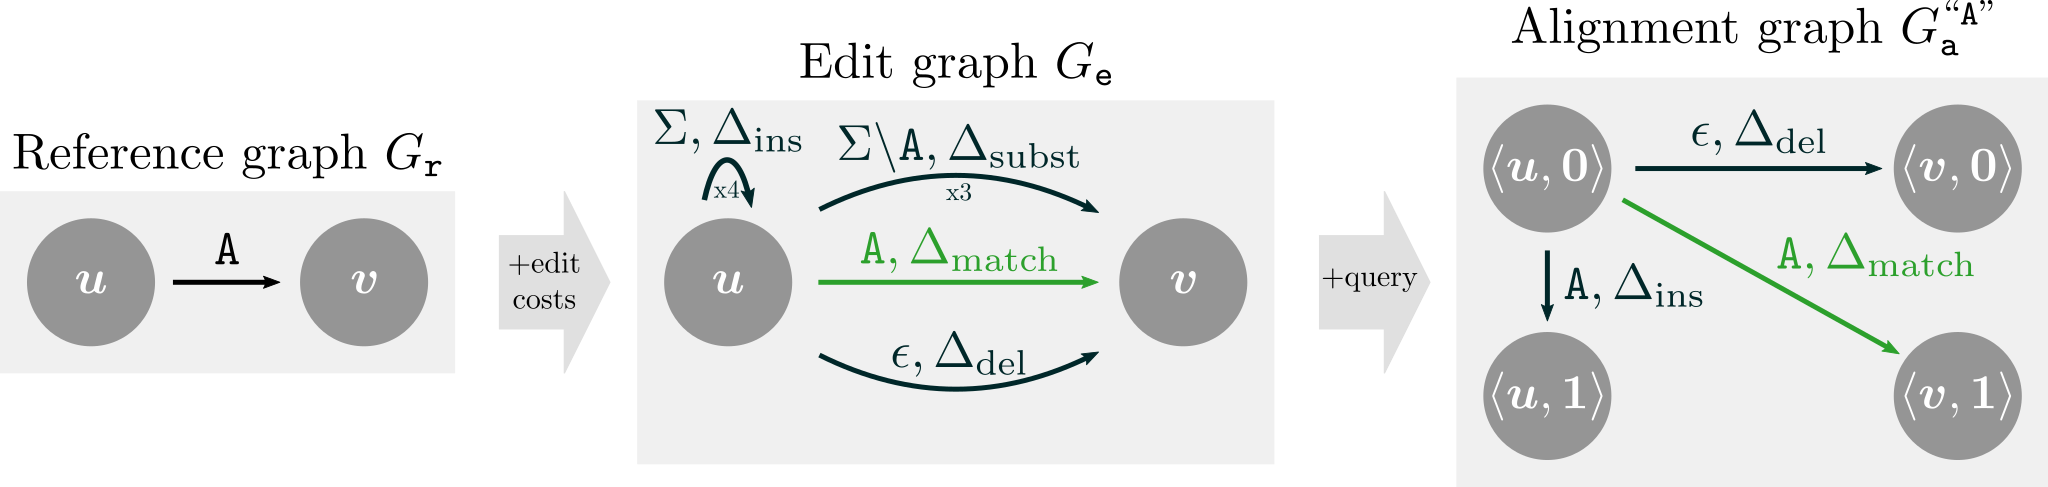
\includegraphics[width=1\columnwidth]{figs/edit_graph}
	\caption[Constructing the alignment graph.]{Starting from the reference graph (left), we can construct the edit graph (middle) and the alignment graph $\AG$ for query $q=``\texttt{A}"$ (right). Edges are annotated with labels and/or costs, where sets of labels represent multiple edges, one for each letter in the set (indicated by $``\text{x}3"$ and $``\text{x}4"$).}
	\label{TRIEfig:graph-constructions}
\end{figure}

\para{Edit Graph}
Instead of representing alignments as pairs of (i)~paths in the reference graph and
(ii)~sequences of edit operations on these paths, we introduce \textit{edit
graphs} whose paths intrinsically capture both. This way, we can
formally define an alignment more conveniently as a path in an edit graph.

Formally, an \emph{edit graph} $\EG:=(\EGV,\EGE)$ has directed, labeled edges
$\EGE \subseteq \EGV \times \EGV \times \Sigma_\epsilon \times \mathbb{R}_{\geq
0}$ with associated costs that account for edits. Here, $\Sigma_\epsilon :=
\Sigma \cup \{\epsilon\}$ extends the alphabet $\Sigma$ by $\epsilon$ to account
for deleted characters (see \cref{fig:graph-constructions}).
%
The edit and reference graphs consist
of the same vertices, \ie, $\EGV=\RGV$. However, $\EGE$ contains more edges
than $\RGE$ to account for edits.
%
Concretely, for each edge $(u,v,\ell) \in \RGE$, $\EGE$ contains edges to
account for (i)~matches, by an edge $(u,v,\ell,\cmatch)$, (ii)~substitutions, by
edges $(u,v,\ell',\csubst)$ for each $\ell' \in \Sigma \backslash \ell$,
(iii)~deletions, by an edge $(u,v,\epsilon,\cdel)$, and (iv)~insertions, by
edges $(u,u,\ell',\cins)$ for each $\ell' \in \Sigma$.
%
The spelling $\sigma(\pi) \in \Sigma^*$ of a path $\pi \in \EG$ is defined
analogously to reference graphs, except that deleted letters (represented by
$\epsilon$) are ignored. The cost $\cost{\pi}$ of a path $\pi \in \EG$ is the
sum of all its edge costs.

\para{Alignment on Edit Graph}
An \emph{alignment} of query $q$ to $\RG$ is a path $\pi \text{ in } \EG$
spelling $q$, \ie, $q=\sigma(\pi)$. An \emph{optimal alignment} is an alignment
of minimal cost.


\paragraph{Alignment Graph}
To find an optimal alignment of $q$ to the edit graph $\AG$ using shortest path
finding algorithms, we must ensure that only paths spelling $q$ are considered.
To this end, we introduce an alternative but equivalent formulation of
alignments in terms of an \emph{alignment graph} $\AG=(\AGV,\AGE)$.

Here, each \emph{state} $\langle v,i \rangle \in \AGV$ consists of a node $v \in
\AGV$ and a query position $i \in \{0,\dots,|q|\}$ (equivalent
to~\cite{rautiainen_aligning_2017}). Traversing a state $\langle v,i \rangle \in
\AGV$ represents the alignment of the first $i$ query characters ending at node $v$.
%
In particular, query position $i=0$ indicates that we have not yet matched any
letters from the query.
%
We note that the alignment graph explicitly depends on the query $q$. In
particular, the example alignment graph $\AG[``\texttt{A}"]$ in
~\cref{fig:graph-constructions} lacks substitution edges from $\AG$, as their
labels ($\texttt{C}$, $\texttt{G}$, $\texttt{T}$) do not match the query
$q=``A"$.

We construct the alignment graph $\AG$ to guarantee that any walk from a source
$\langle u,0 \rangle$ to a state $\langle v,i \rangle$ corresponds to an
alignment of the first $i$ letters of query $q$ to $\RG$. As a consequence,
there is a one-to-one correspondence between alignments $\pi$ of $q$ to
$\AG$ and paths $\alignment{\pi} \in \AG$ from sources $S:=\RGV \times \{0\}$ to
targets $T:=\RGV \times \{|q|\}$, with
$\cost{\reference{\pi}}=\cost{\alignment{\pi}}$. To find the best alignment in
$\AG$, only paths in $\AG$ (walks without repeating nodes) can be considered,
since repeating a node in $\AG$ cannot lead to a lower cost ($\cdel \geq 0$) for
the same state.

\begin{samepage}
The edges $\AGE \subseteq \AGV \times \AGV \times \Sigma_\epsilon \times
\mathbb{R}_{\geq 0}$ are built based on the edges in $\AGE$, except that the
former (i)~keep track of the position in the query $i$, and (ii)~only contain
empty edges or edges
whose label matches the next query letter:

\vspace{-0.7em}
{%
\small
\begin{alignat}{10}
	(u,v,\ell,w) &\in \AGE \implies (&\langle u, i \rangle, &\langle v, i+1
		&&\rangle,\ell,w) \in \AGE \quad \text{ for } 0 \leq i < |q| \text{ with }
		q[i]=\ell \label{eq:alignment-edges-nondeletions} \\
	(u,v,\epsilon,w) &\in\AGE \implies (&\langle u, i \rangle, &\langle v, i
		&&\rangle,\epsilon,w) \in \AGE \quad \text{ for } 0 \leq i < |q| \label{eq:alignment-edges-deletions}
\end{alignat}
}%
\end{samepage}
%
Here, assuming $0$-indexing, $q[i]$ is the next letter to be matched after
matching $i$ letters. Then, \cref{eq:alignment-edges-nondeletions} represents
matches, substitutions, and insertions (which advance the position in the query
by $1$), while \cref{eq:alignment-edges-deletions} represents deletions (which do
not advance the position in the query).

\paragraph{Dynamic Construction}
As the size of the alignment graph is $\Oh(\lvert \RG \rvert \concat \lvert q
\rvert)$, it is expensive to build it fully for every new query.
Therefore, our implementation constructs the alignment graph $\AG$ on-the-fly:
the outgoing edges of a node are only generated on demand and are freed from
memory after alignment.
